% Chapter 3

\chapter{Implementation} % Main chapter title

\label{Chapter3}

We will now look upon the implementation of the aforementioned changes. Unlike to the original
implementation this is not a C library, but a pure Haskell library. This brings some advantages 
and one disadvantages. The disadvantage is the performance as discussed in \textbf{REF TO EVALUATION}.
For the costs of performance we gain a library that is easy to understand and extend. The original 
implementation is interwoven with the GHC runtime environment. Some STM functions are evoked by 
the scheduler to ensure the consistency. This makes the library sensitive to changes. 
To ensure the correctness of such a library is significantly harder than with a pure library, since
the compiler does not aid this porcess. In other words, the devlopment of a pure library is safer
and faster. \parencite{STMHigh} presented a high level Haskell implementation of STM. Their aim
was to provide a pure Haskell implementation that is equivalent to original implementation of 
\parencite{STMBase}. Preceding this master thesis I optimized that implementation. I replaced
internally used data structure and performed two changes to the internal semantics. First, 
the initial high level implementation used a global lock to synchronize concurrent transactions.
This coarse grained locking was substituted by an fine grained locking. Instead of a single
global lock, each TVar holds its own lock and transactions acquire the minimum amaunt of 
locks to commit. This prevents transactions, that do not conflict, to commit simultaneously.
Second, I altered the conflict detection. The initial implementation used a validation process
similar to the GHC implementation. Each TVar has a queue associated. If a transaction reads this 
a TVar, it enters a reference to itself. If a transaction successfully commits a change to a TVar it 
notifies all transactions in the associated queue. If a transaction is notified it is rolled back.
This way of conflict detection has the advantage that conflicts are detected earlier than before.
This implementation is called the \keyword{project implementation} in the following. Figure 
\ref{fig:implementations} visualizes the development process of the libraries.
We will now head over to a detailed description of the implementation developed in the course of this 
thesis. 

\begin{figure}
\centering
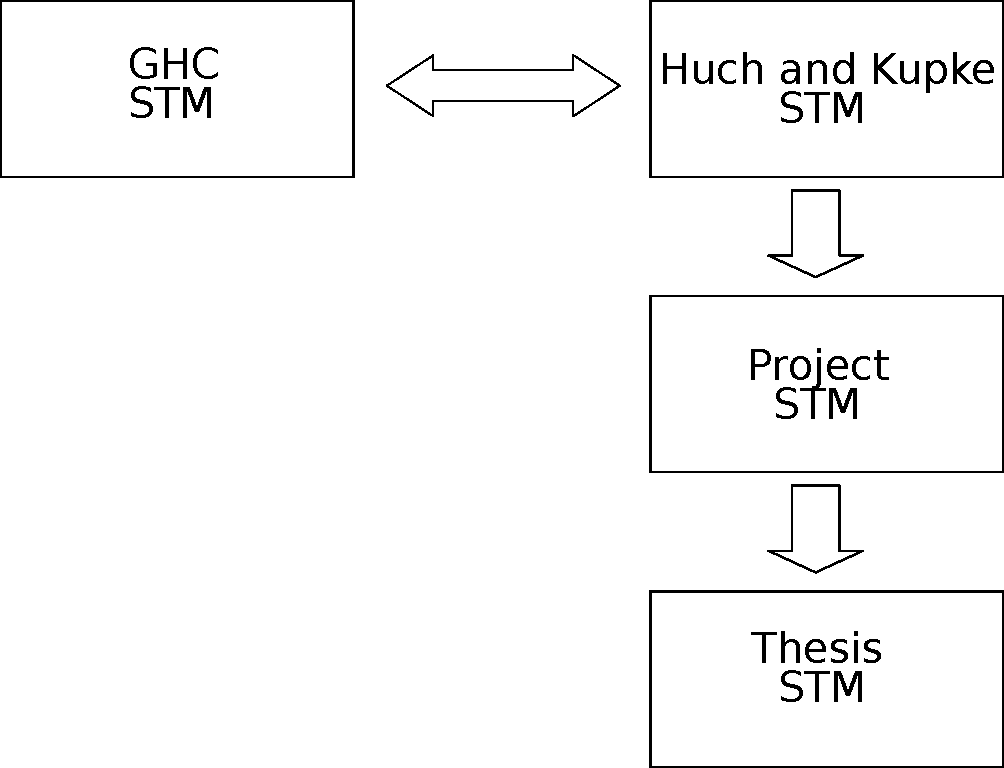
\includegraphics[scale=0.8]{Figures/implementations}
\decoRule
\caption[implementations]{The STM implementations for Haskell.}
\label{fig:implementations}
\end{figure}

\section{STM Types}
Before we head over to the implementation of the external interface of STM, we investigate the types
of STM that are used in this implementation starting with the STM type itself:
\begin{lstlisting}
 data STM a = STM (StmState -> IO (STMResult a))
\end{lstlisting}
In its core the STM data type is a state monad. The IO type on was initially needed to perform the reads 
in the computation phase. As we will see later this implementation needs the IO only to create new TVars
in the computation phase. \code{readTVar} and \code{writeTVar} do not need IO operations to be processed.
Thus an STM action takes a state and returns a result depending on this state. There are three possible 
results:
\begin{lstlisting}
 data StmResult a = Retry StmState
                  | InValid
                  | Success StmState (Maybe a)
\end{lstlisting}
The first constructor is used to indicate that a \code{retry} occurred. This must be distinguished from 
\code{InValid}, since \code{orElse} and \code{atomically} react differently on these results. If 
\code{Retry} is returned, \code{atomically} validates and rolls back if needed and \code{orElse} 
would start the second transaction. This is the reason \code{Retry} is accompanied by the state.
The state hold the necessary information about the TVars the transaction has read. This allows 
to validate and possibly suspend on particular TVars. \code{InValid} on the otherhand is indicates
always that the transaction is not valid and thus must be restarted. 
The last constructor is the desired outcome of an action. If the transaction does not fail, it returns
\code{Success} and a state as well as the result. As before the state is needed for validation.
The result is wrapped by the \code{Maybe} type. The value \code{Nothing} never occurs. 
The reason for this wrapping is explained in Section \ref{sec:IFFun}. 

Before we examine the StmState, we need to take a look at the \code{TVar}
\begin{lstlisting}
 data TVar a = TVar (MVar (IORef a))
                    ID
                    (MVar [MVar ()])
                    (MVar ())
\end{lstlisting}
All TVars have a globally unique identifier called \code{ID}, which is immutable. The \code{MVar (IORef a)} 
hold the actual value of the TVar. The MVar is used to synchronize multiple transaction, if they intend to 
access the same TVar. The \code{IORef} is needed to enable a correct validation, which is explained in detail
in \ref{sec:IFFun}. \code{MVar [MVar ()]} is the queue of the MVar where transactions that wait on a change
enter their their personal \code{MVar ()}. Remember that this is needed to delay the rollback when retry
is evoked. The last part is an explicit lock for this TVar. There are currently two implementations as 
a result of this thesis. The details are explained later. One of these implementations lock a TVar via 
the explicit lock and the other by taking the MVar that hold the value.

The only thing that happens in the computation phase is that the \code{StmState} is computed.
The core data structure is the \code{StmState} which holds all informations to process a transaction:
\begin{lstlisting}
 data StmState = TST {writeSet   :: IntMap (Maybe (),
                                            Maybe (),
                                            MVar (IORef ())),
                      notifies   :: IO (),
                      readSet    :: ReadSet,
                      retryMVar  :: MVar (),
                      uEReads    :: [Maybe ()]}
\end{lstlisting}
The \code{writeSet} is similar to the log in the GHC implementation. It is a \code{IntMap} 
\footnote{This refers to the IntMap in the standart libraries of Haskell: \url{https://hackage.haskell.org/package/containers-0.5.8.1/docs/Data-IntMap-Strict.html}}. 
The keys are the IDs of the associated TVars. The elements contain the \code{expectedValue},
the \code{newValue}, and \code{actualMVar}. The \code{actualMVar} is needed in the commit
phase when the transaction sucessfully commits to publish its modifications. We know already the 
\code{expectedValue} and the \code{newValue} from \ref{sec:GHCImpl}, but their purpose is slighty 
different. The \code{Maybe} type indicates that the values also can be \code{Nothing}. This holds
only for the second entry. The first entry has the \code{Maybe} type for the same reason the 
\code{Success} has it. The second entry on the other hand can become \code{Nothing}. This indicates
that the TVar was read but not written by the transaction. Note that there are two kinds of 
\textit{read}. The first is that \code{readTVar} operation is porcessed in the computation phase
and the second that the current value of the TVar was read. In the original implementation these 
two occur always at the same time. In the new approach theses kinds of reads occur at different.
For clearity I will from now on say IO-reads when I refer to a read from the actual IORef to access
the current value of that TVar. 

\code{nofifies} holds an IO action that is process when the transaction successfully commits.
This IO action notifies all transactions that are waiting on a TVar that is modified by the 
committing transaction.

\code{readSet} stores information about the IO-reads that where performed. \code{ReadSet}
is defined as follows:
\begin{lstlisting}
 type ReadSet = IORef (InMap (IORef (), 
                              MVar (IORef ()), 
                              MVar [MVar ()]))
\end{lstlisting}
The need for the outermost IORef is explained later. This type is like the \code{writeSet} an 
\code{IntMap}. The keys are the IDs of the TVars. The entries consist of three parts. First,
the value (in form of the IORef) that was present when the IO-read was executed. Second, the 
MVar the IORef that holds the value was read from. Third, the queue of the associated TVars.
The exact ussage of this is explained in the next section.

\code{retryMVar} is a unique MVar for every transaction. This is the MVar that is entered into
the queues of the TVars when needed.

\code{uEReads} contains all unevaluated IO-read operations. This is essential to be able to 
process the IO-reads that where not evaluated in the computation phase. The \code{Maybe} type
is again for the same reasons used as it is in \code{StmResult}.

This concludes the overview on the data structures used and we can now head over to see how these
data structures are used to implement the STM interface.





\section{Interface Functions}
\label{sec:IFFun}












\section{lock write is enough}

\subsection{MOVE THIS TO THE IMPLEMENTATION CHAPTER}
When the commit phase begins the transaction is validated. The validation does not differ from the validation 
in the original implementation. When a \code{readTVar} is evaluated the current value of the TVar is logged. 
Validating the transactions means to check if the logged values match the current values of the TVars. 
If the transaction is not valid, it is rolled back.
If the transaction is valid, the TVars that the transaction want to modify are locked and the transactions is validated again. 
This is needed, because it is possible that a TVar in the log was modified after the validation and before 
the lock was acquired. This seems to be an unnecessary overhead, but has a slightly better performance than first 
locking and then validating. This is discussed in Chapter\textbf{REF TO EVALUATION}. The original implementation 
also uses this scheme, which was proposed by Fraser \parencite[Page 42]{lockfreedom}. The reason is
the cost for locking the TVars. This locking itself is not particular expensive, but it hinders parallelism.
Everytime a TVar is locked no other transaction is able to read, lock, or validate this TVar. Additionally if 
a TVar tries to access a locked TVar, it is suspended and a context switch follows. Context switches in Haskell 
are not as expensive as context switches of OS threads, but it schould not be neglected, especially when dealing
with a large number of threads. Validation is a operation, which needs two memory access per entry in the log.
One memory access is the access to the log entry to look up the expected value and the other memory access is
the access to the actual TVar\footnote{The log entry needs to be accessed two times. First to get the expected
value and second to get the next entry, because the log is a dynamic structure and thus needs a pointer
to the next entry comparable to a list. Nevertheless the entry itself is (most likely) in one block in the memory.
This is why I consider one memory access to be enough for the entry.}. This is reasonable considering that the 
log only consists of TVars that are needed to determine the control flow. So validation is significant faster
than locking. 

% After the locks has been acquired and the log was validated, the remaining \code{readTVar} operations are evaluated.

At this point no other transaction is able to modify the TVars and thus the evaluation is safe in the sense
that the value cannot change until the commit of the transaction is completed. After the reads are evaluated the 
writes are processed and the result is returned after unlocking the TVars.

%TODO example


